
\section{HTTP}

\subsection{Скриншоты}

\begin{center}

    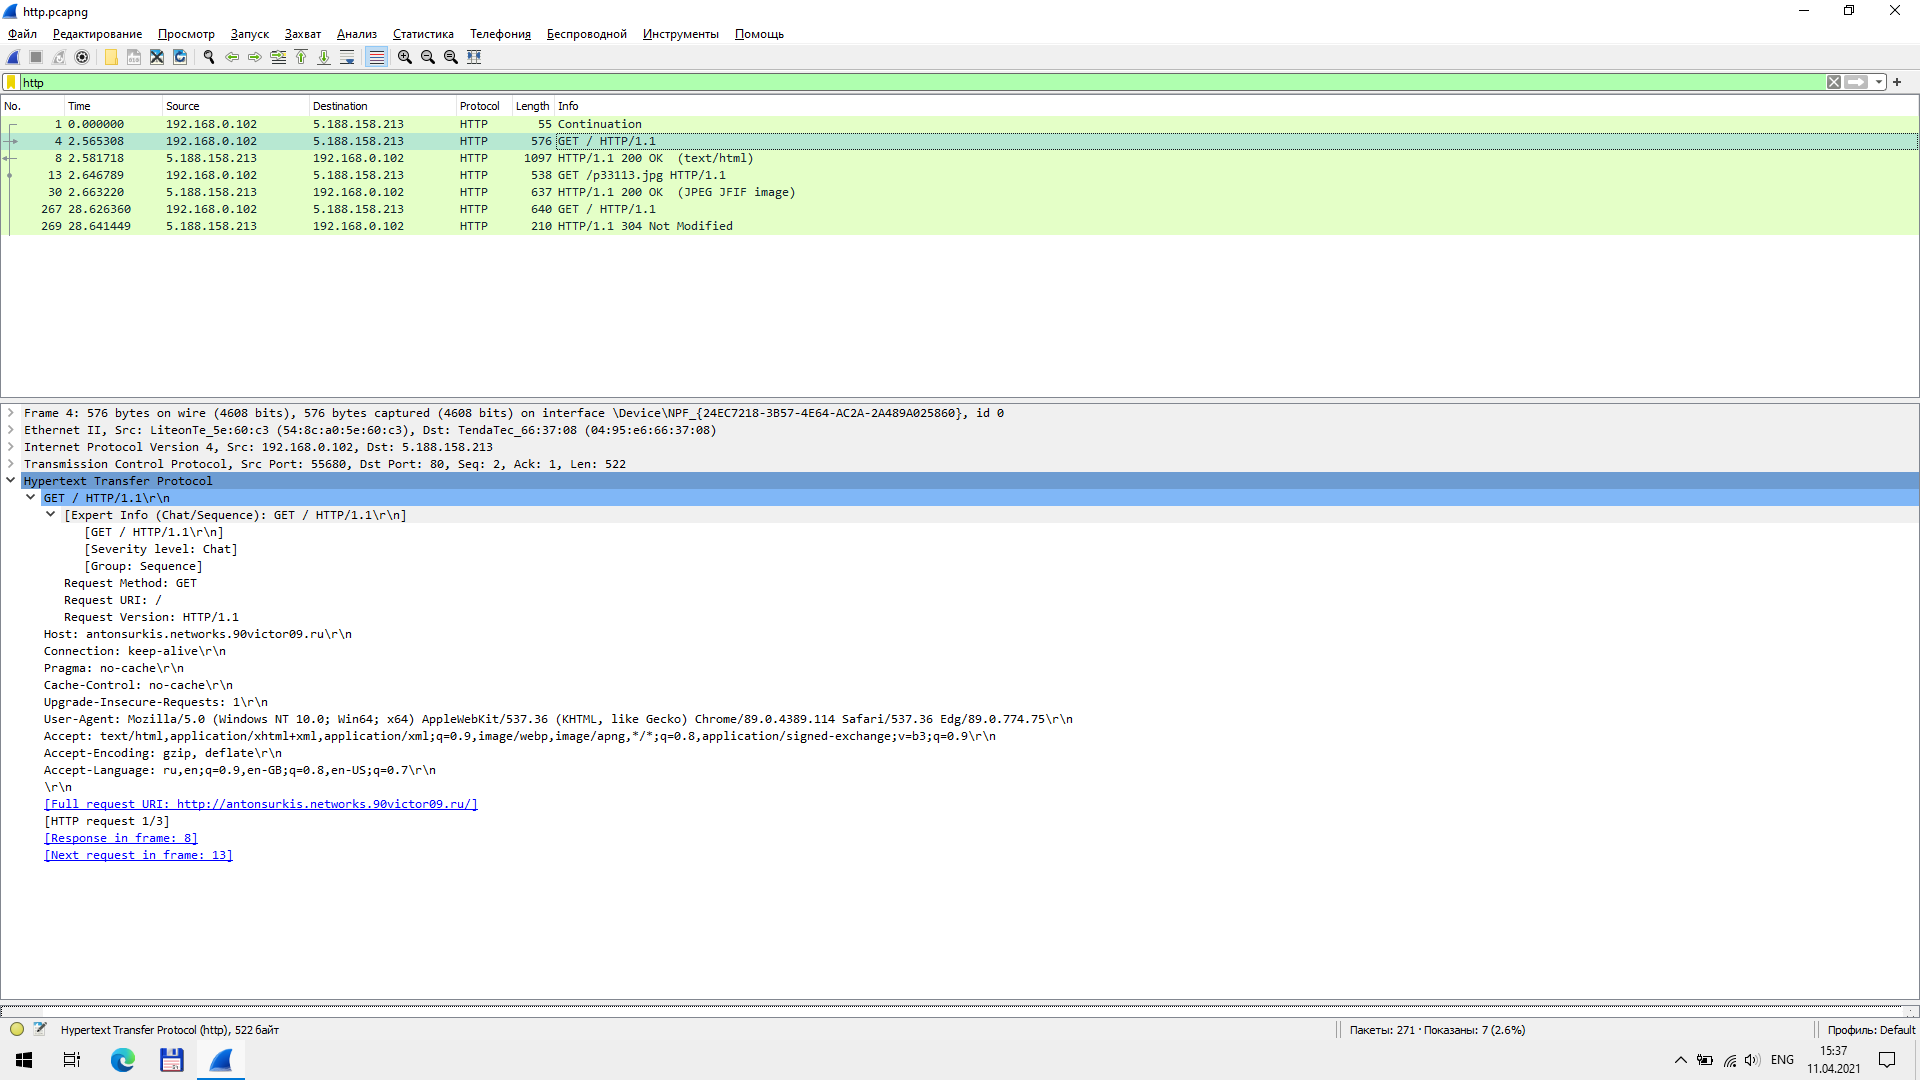
\includegraphics[width=\textwidth]{screenshots/http_get_text_request_1}

    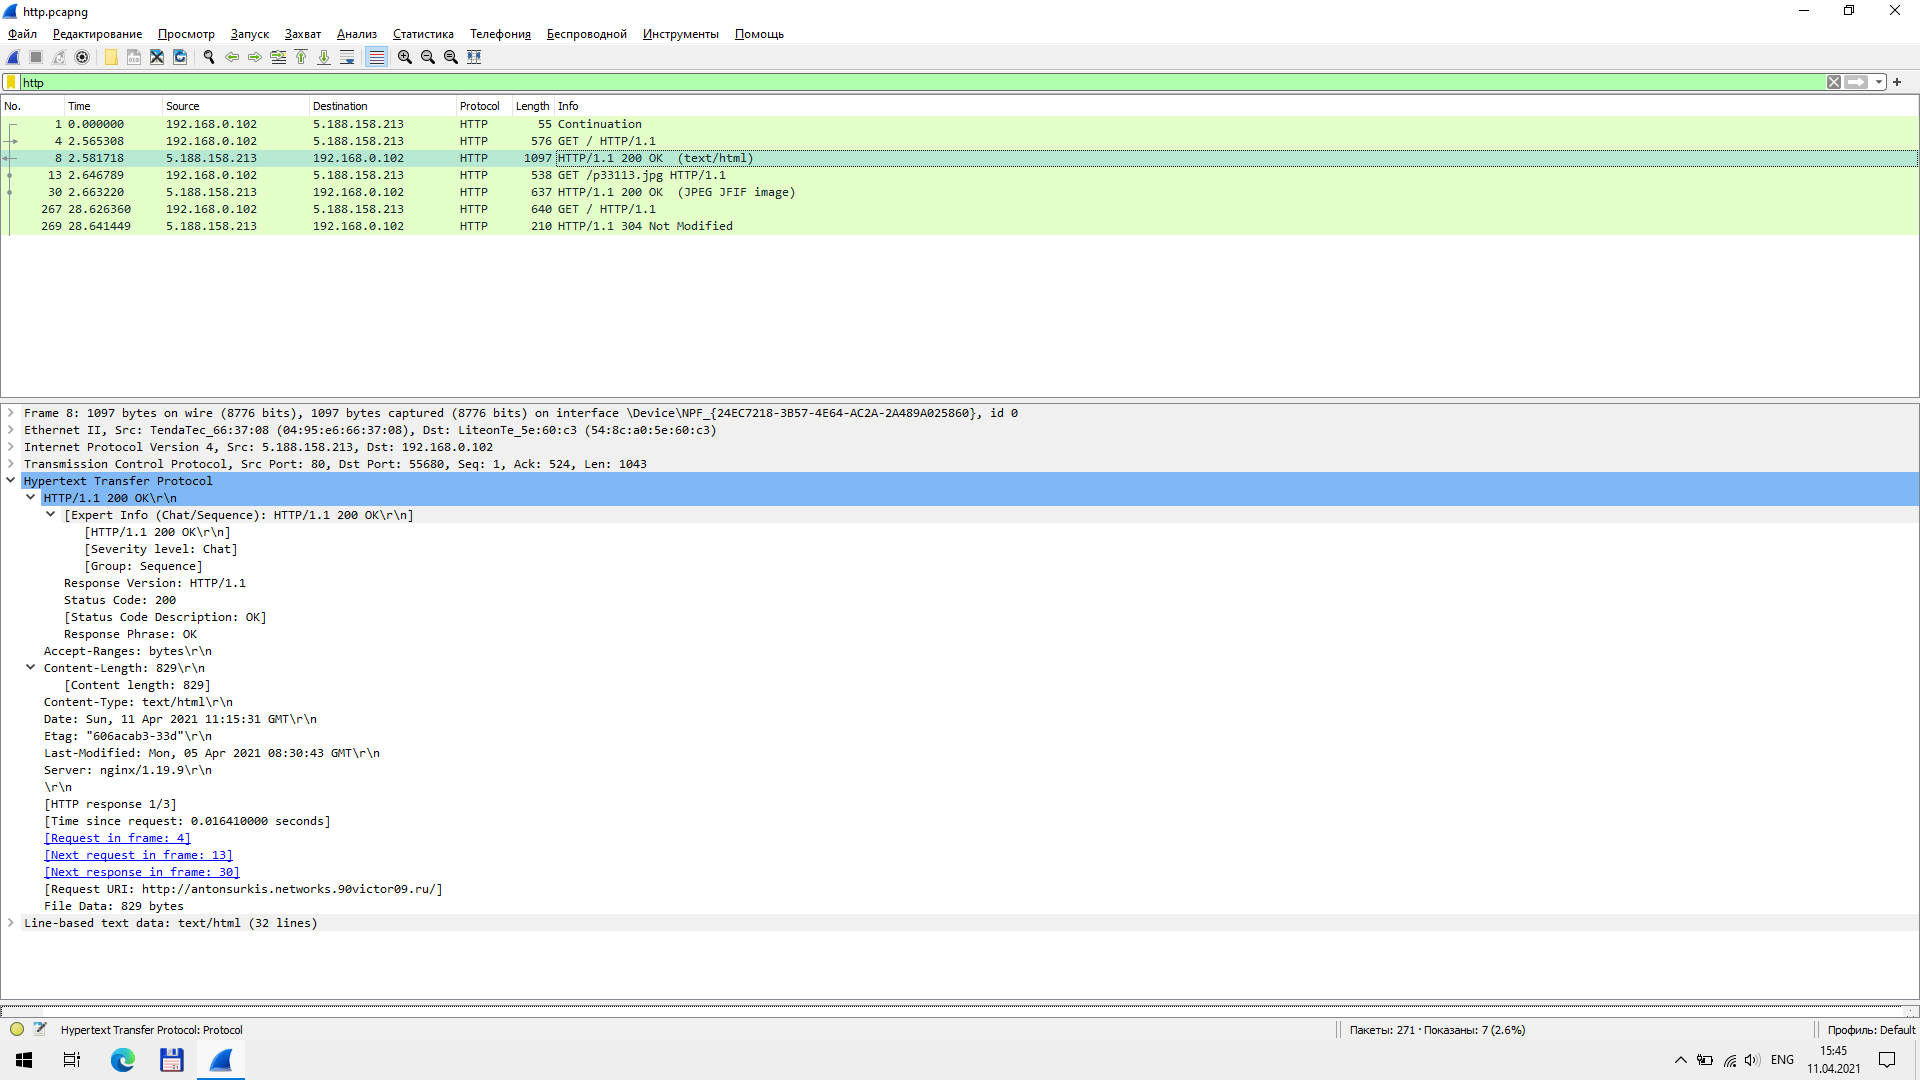
\includegraphics[width=\textwidth]{screenshots/http_get_text_response_1}

    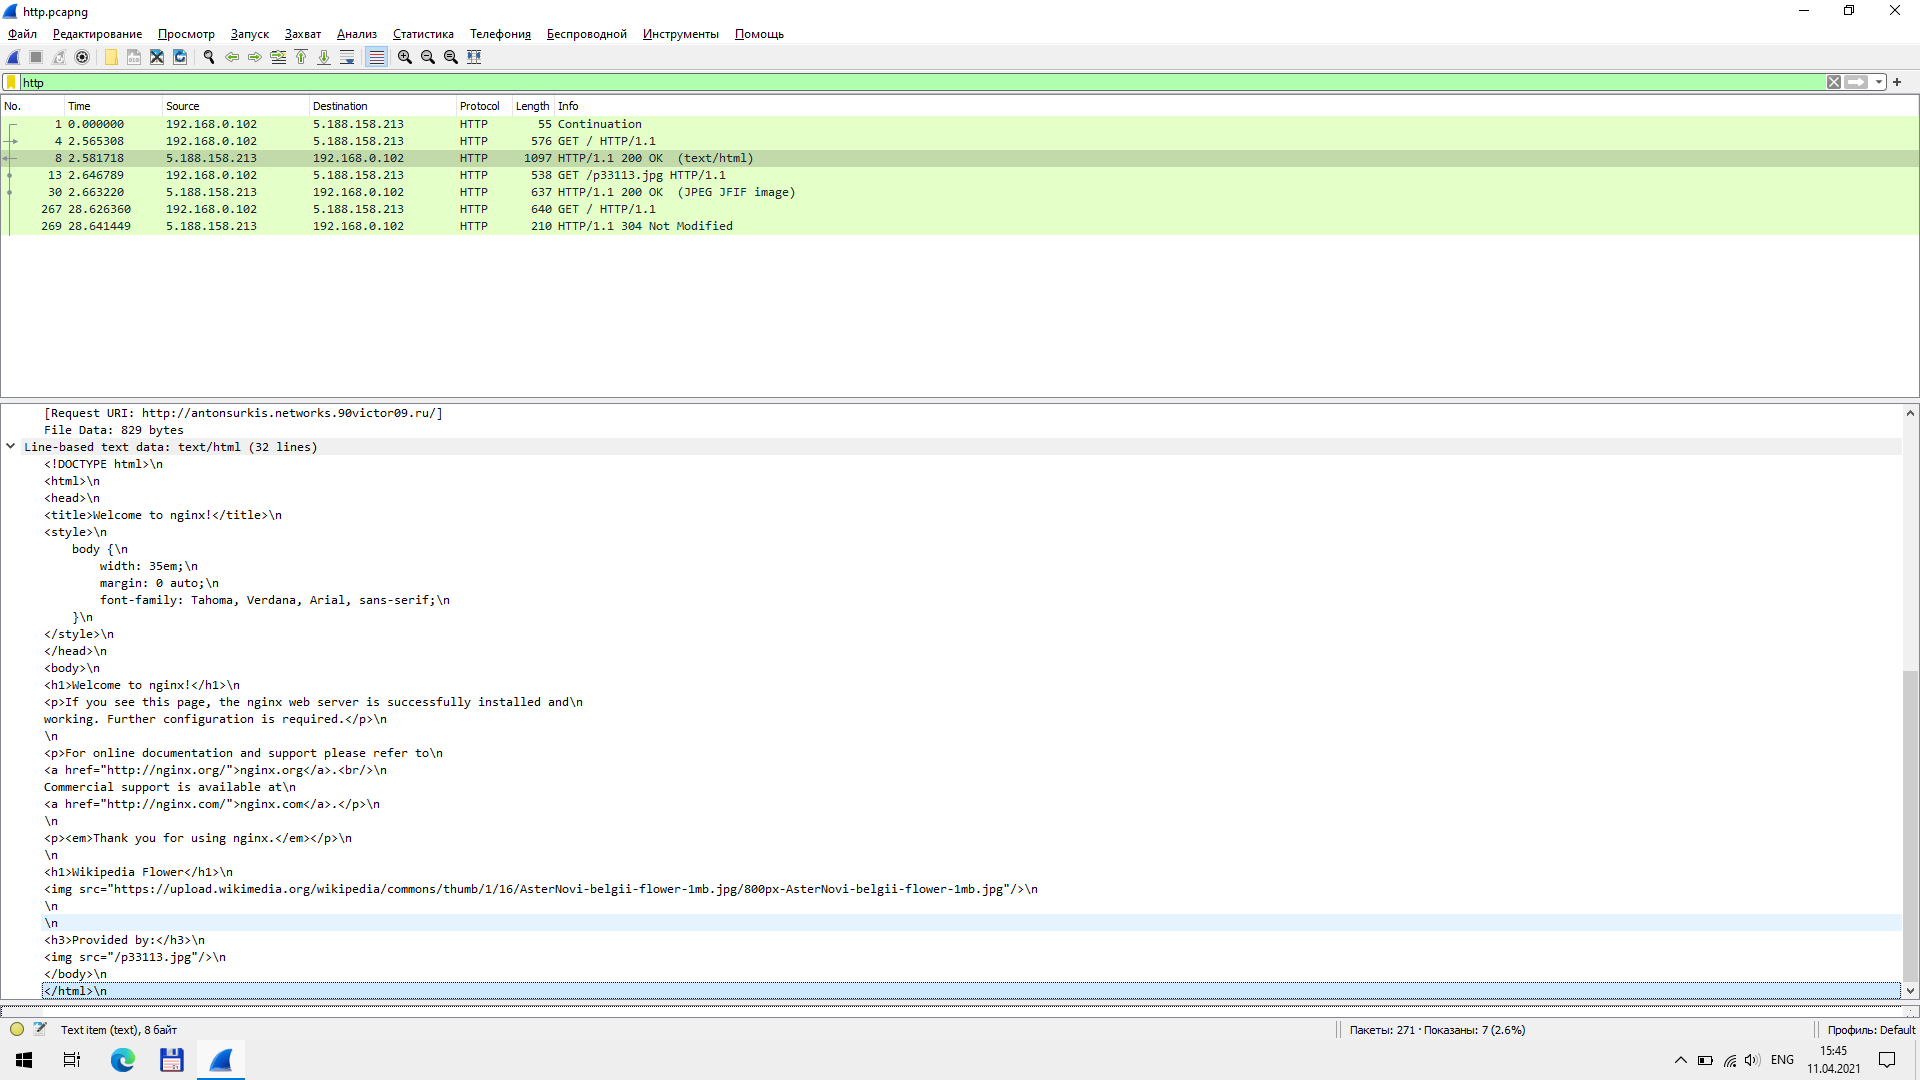
\includegraphics[width=\textwidth]{screenshots/http_get_text_response_2}

    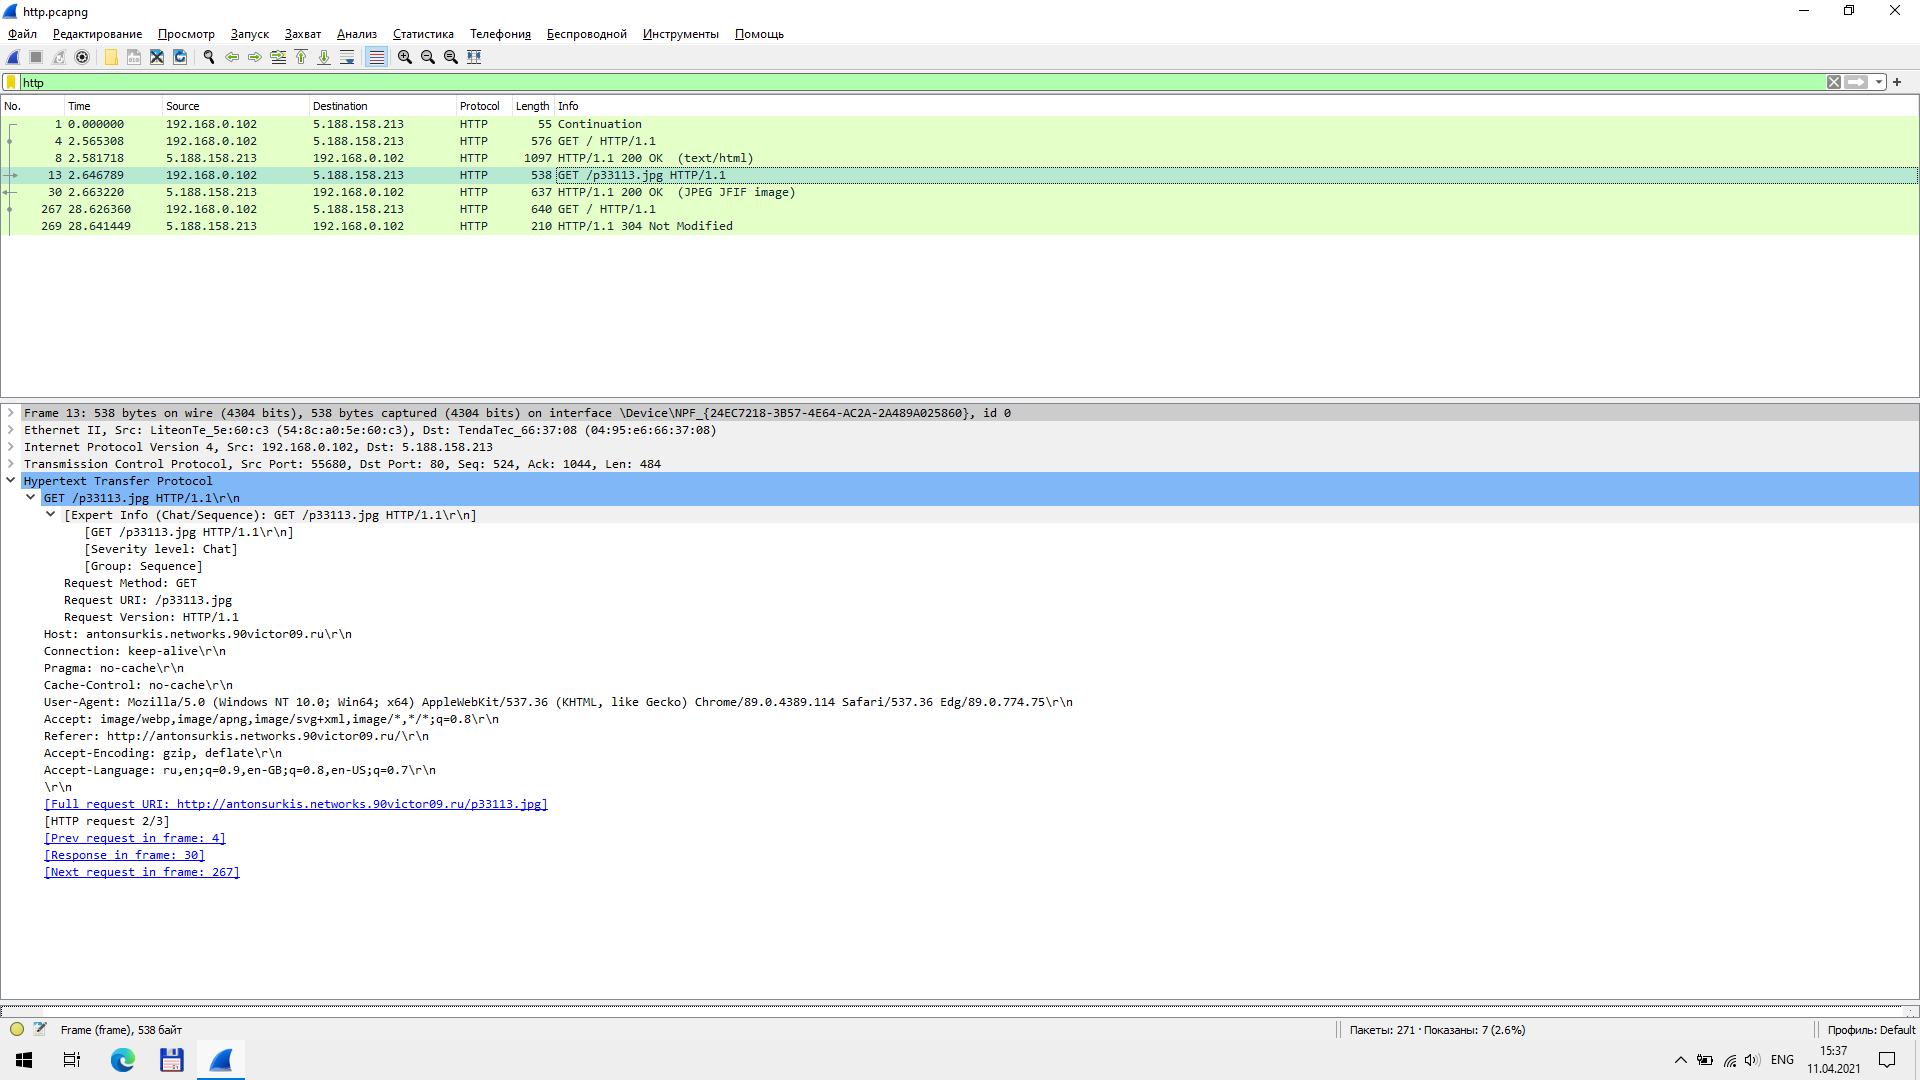
\includegraphics[width=\textwidth]{screenshots/http_get_jpg_request_1}

    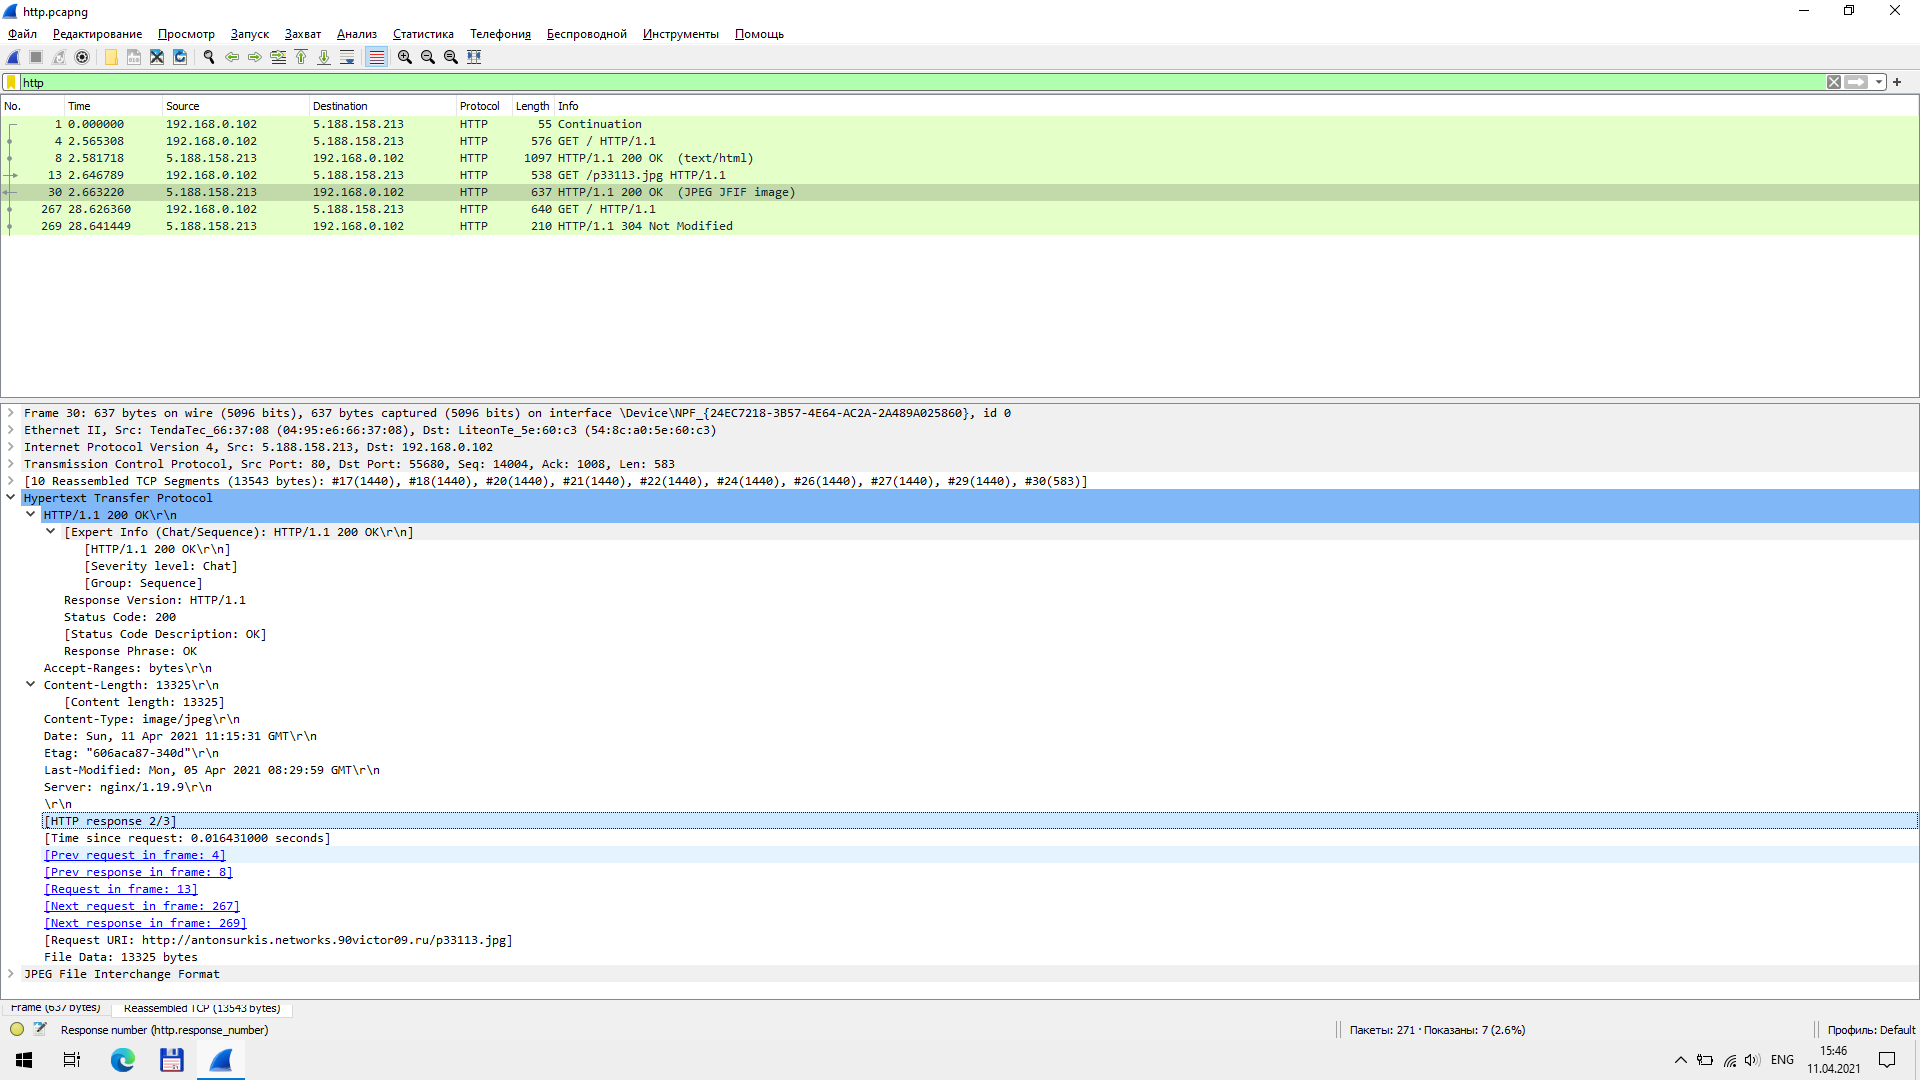
\includegraphics[width=\textwidth]{screenshots/http_get_jpg_response_1}

    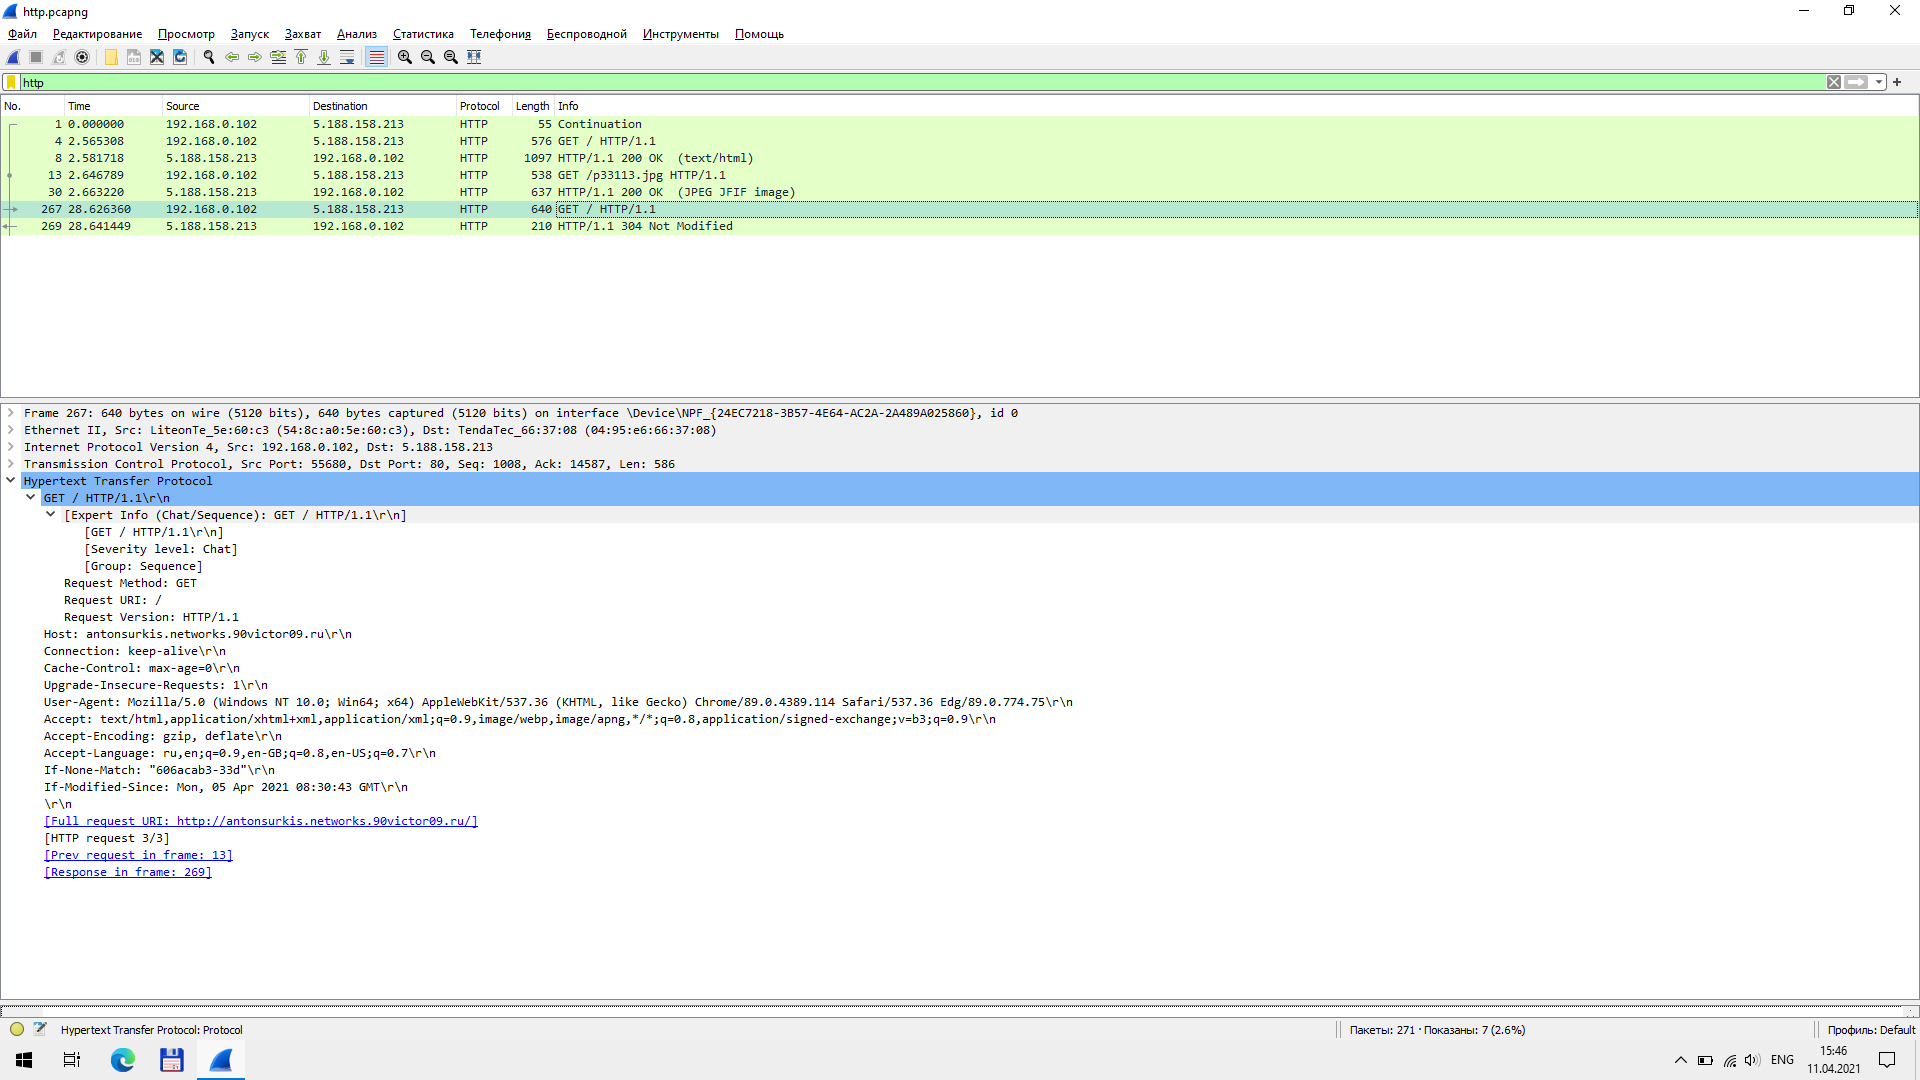
\includegraphics[width=\textwidth]{screenshots/http_get_cached_request_1}

    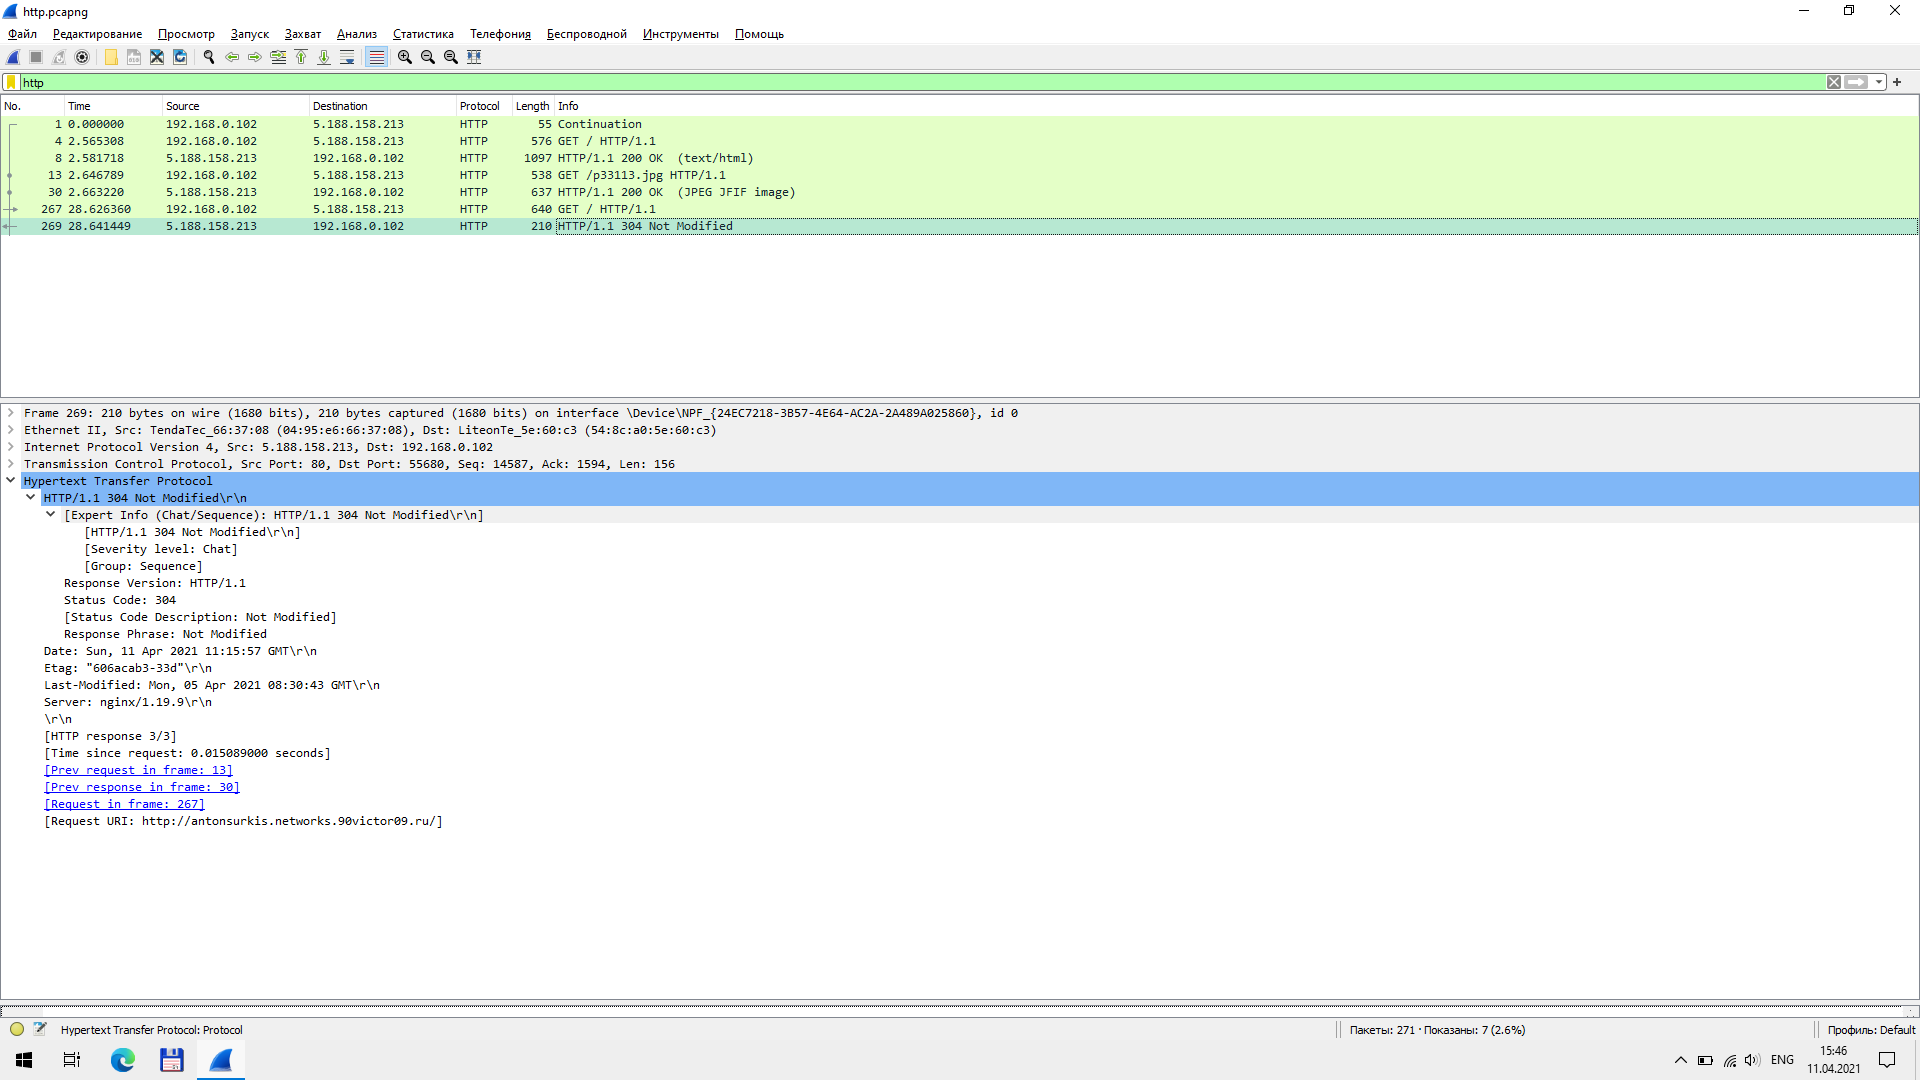
\includegraphics[width=\textwidth]{screenshots/http_get_cached_response_1}

\end{center}

\subsection{Ответы на вопросы}

При первичном обращении браузер генерировал HTTP-запрос с
\texttt{Pragma: no-cache} и \texttt{Cache-Control: no-cache}.
После получения ответа в виде HTML-страницы парсил ее и запрашивал изображение.
Оба ответа были с кодом 200.

При вторичном обращении браузер генерировал HTTP-запрос без
\texttt{Pragma} и с \texttt{Cache-Control: max-age=0},
\texttt{If-None-Match: "606acab3-33d"} и
\texttt{If-Modified-Since: Mon, 05 Apr 2021 08:30:43 GMT}.
Получив ответ с кодом 304 браузер полность отобразил страницу из кеша.
